\section{Lecture 2: Basic Concepts}
\begin{itemize}
    \item Suppose we have a system in equilibrium with three forces acting on it. We have three weights $W$ pulling down on massless wires, two of which loop through a pulley to hold the center mass in equilibrium.
    \begin{center}
        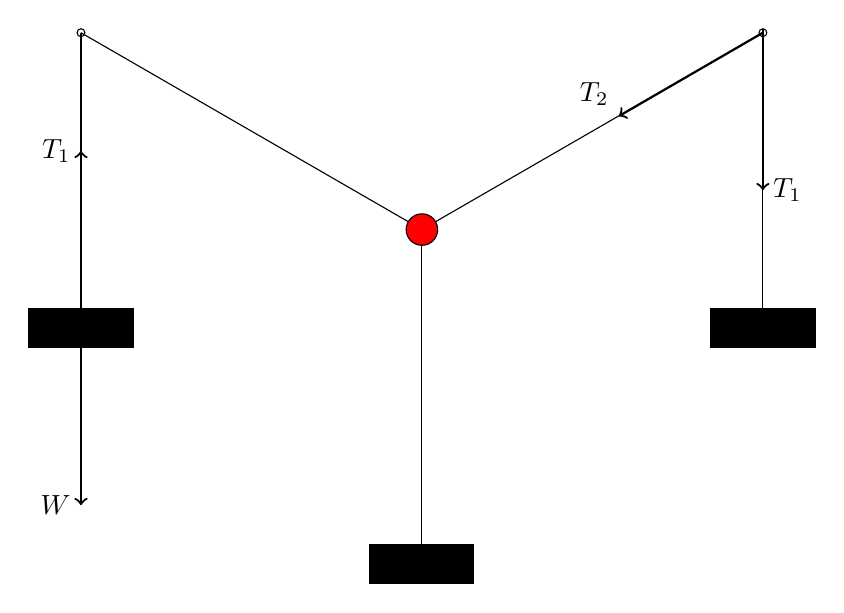
\begin{tikzpicture}            
            \draw[] (0,0) -- (4.33,2.5);
            \draw[] (4.33,2.5) circle (0.05);
            \draw[] (4.33,2.5) -- (4.33,-1);
            \draw[->,thick] (4.33,2.5) -- (2.5,1.44) node[above left] {$T_2$};
            \draw[->,thick] (4.33,2.55) -- (4.33,0.5) node[right] {$T_1$};

            \draw[fill=black] (3.66,-1) rectangle (5,-1.5);
    

            \draw[] (0,0) -- (-4.33,2.5);
            \draw[] (-4.33,2.5) -- (-4.33,-1);
            \draw[fill=black] (-3.66,-1) rectangle (-5,-1.5);

            \draw[] (-4.33,2.5) circle (0.05);
            \draw[] (0,0) -- (0,-4);
            \draw[fill=black] (-0.66,-4) rectangle (0.66,-4.5);

            \draw[->,thick] (-4.33,-1.25) -- (-4.33,-3.5) node[left] {$W$};
            \draw[->,thick] (-4.33,-1.25) -- (-4.33,1) node[left] {$T_1$};
            \draw[fill=red] (0,0) circle (0.2);
        \end{tikzpicture}
    \end{center}
    \item To determine the forces in the wires, we draw a free body diagram on any weight, to get:
    \begin{equation}
        T_1 = W
        \label{eq:}
    \end{equation}
    \item The moment (or torque) is defined as the cross product between a position vector and the force vector\footnote{In a flat plane, $M$ is instead a pseudovector (behaves like a scalar) and it is not necessary to write the vector symbol.}:
    $$\vec{M}=\vec{r}\times \vec{F}$$
    \item Using this we can balance moments on each pulley of radius $R$:
    \begin{equation}
        T_1R=T_2R \implies T_1=T_2
        \label{eq:}
    \end{equation}
    Note that the force of tension at the bottom is equal to the tension force at the top since the wire is assumed to be massless.
    \item Therefore, the three tension forces acting on the center mass are equal. We can balance forces in the $x$ and $y$ directions:
    \begin{align}
        \sum F_y = 0 = T\cos\alpha-T\cos\beta \\ 
        \sum F_y = 0 = T\sin\alpha+T\sin\beta-T 
    \end{align}
    where $\alpha$ and $\beta$ are the angles the top two wires make with the horizontal. solving this system gives us:
    \begin{equation}
        \alpha=\beta=30^\circ
        \label{eq:}
    \end{equation}
    In other words, the force vectors form an equilateral triangle when arrange tip to tail.
    \item However in reality, $\alpha=\beta$ are slightly larger than $60^\circ$, caused by the extra downwards force caused by the mass of the washer and strings (which we did not include in our analysis)
    \item Suppose two people play a game of tug of war as shown in the image below where the tensile force is $T=100 \text{ N}$
\begin{center}
\begin{tikzpicture}[line cap=round,line join=round,>=triangle 45,x=1cm,y=1cm]
\draw [rotate around={90:(-5.56,4.74)}] (-5.56,4.74) ellipse (0.6138958458972931cm and 0.6020532448296847cm);
\draw [rotate around={-63.434948822921996:(-4.5,3)}] (-4.5,3) ellipse (1.3884124055004496cm and 0.8232186876811883cm);
\draw [] (-4.3630522255092945,1.7515683312019743)-- (-3.2,0.1);
\draw [] (-3.5620615429182125,2.2246565488811223)-- (-2.34,0.56);
\draw [] (-2.34,0.56)-- (-1.84,0.56);
\draw [] (-3.2,0.1)-- (-2.64,0.1);
\draw [rotate around={63.43494882292203:(3.5,3)}] (3.5,3) ellipse (1.4221336636241415cm and 0.8788994010767188cm);
\draw [rotate around={61.18920625702733:(4.55,4.82)}] (4.55,4.82) ellipse (0.6549998899524413cm and 0.6139420622808884cm);
\draw [] (3.363703512297522,1.708524134155108)-- (2,0);
\draw [] (2,0)-- (1.4,0);
\draw [] (2.544627980791673,2.127868612215594)-- (1.58,0.86);
\draw [] (1.58,0.86)-- (1.08,0.86);
\draw [] (-4.82,3.52)-- (-4.52,3.28);
\draw [] (-4.52,3.28)-- (-3.04,3.34);
\draw [] (3.76,3.6)-- (3.38,3.26);
\draw [] (3.38,3.26)-- (2.08,3.28);
\draw [,color=blue] (-3.0585265604964977,3.339248923223115)-- (2.08,3.28);
\draw [->,color=blue] (0.20348486424459367,3.533552141141065) -- (2.2034848642445946,3.533552141141065) node[midway, above] {$100 \text{ N}$};
\draw [->,color=blue] (-1.1614186509519226,3.60670221755838) -- (-3.1614186509519238,3.60670221755838) node[midway, above] {$100 \text{ N}$};
\begin{scriptsize}
\draw [fill=blue] (-3.0585265604964977,3.339248923223115) circle (2.5pt);
\draw [fill=blue] (2.08,3.28) circle (2.5pt);
\end{scriptsize}
\end{tikzpicture}
\end{center}
Since the rope is in equilibrium, the two forces the two people exert must be equal to each other. Now let us look at the equilibrium of the person to the left (Bill):
\begin{center}
\begin{tikzpicture}[line cap=round,line join=round,>=triangle 45,x=1cm,y=1cm]
\draw [rotate around={90:(-5.56,4.74)}] (-5.56,4.74) ellipse (0.6138958458972931cm and 0.6020532448296847cm);
\draw [rotate around={-63.434948822921996:(-4.5,3)}] (-4.5,3) ellipse (1.3884124055004496cm and 0.8232186876811883cm);
\draw [] (-4.3630522255092945,1.7515683312019745)-- (-3.2,0.1);
\draw [] (-3.5620615429182125,2.2246565488811223)-- (-2.34,0.56);
\draw [] (-2.34,0.56)-- (-1.84,0.56);
\draw [] (-3.2,0.1)-- (-2.64,0.1);
\draw [] (-4.82,3.52)-- (-4.52,3.28);
\draw [] (-4.52,3.28)-- (-3.04,3.34);
\draw [->,color=blue] (-3.0585265604964977,3.339248923223115) -- (-1.2287551766311509,3.3323894309934468) node[midway,above] {$T=100 \text{ N}$};
\draw [->,color=red] (-4.53879613451468,2.9300640106982114) -- (-4.557083653619009,0.8087117945960607)node[left] {$W=1000 \text{ N}$};
\draw [->,color=red] (-2.746619262290449,-1.422365536132063) -- (-2.723488111807894,0.3782917064187159)node[midway,left] {$F_N$};
\draw [->,color=blue] (-1.2341095786520513,0.37829170641871596) -- (-2.723488111807894,0.37829170641871596)node[midway,below] {$F_s$};
\begin{scriptsize}
\draw [fill=blue] (-3.0585265604964977,3.339248923223115) circle (2.5pt);
\end{scriptsize}
\end{tikzpicture}
\end{center}
\item From balancing forces in orthogonal directions, we can see that $F_s=T=100 \text{ N}$ and $F_N=W=1000 \text{ N}$.
\item There is also a balance of torque. A \textbf{couple} is a pair of forces with equal magnitude and opposite direction that act on a different line of action (causing a net moment).
\item The moment of the $F_s$ and $T$ couple is (assuming the perpendicular distance between them is $1.5 \text{ m}$)
\begin{equation}
    M= 100 \times 1.5=150 \,\mathrm{N\cdot m} \text{ [CW]}
    \label{eq:}
\end{equation}
\item The moment of the $W$ and $F_N$ couple must also be $M$. If the horizontal between the center of gravity and the feet is $L$, then we have:
\begin{equation}
    1000 \times L = 150 \implies L = 0.15 \text{ m}
    \label{eq:}
\end{equation}

\begin{theorem}
    In a system with $N$ couples, then the sum of the moments of all the couples have to sum up to zero. In other words, for any reference point, the net torque due to a couple is invariant.
    \vspace{2mm}

    To prove this, consider the torque due to an arbitrary couple about a coordinate $O$ as shown in the diagram below:
    \begin{center}
        \begin{tikzpicture}[line cap=round,line join=round,>=triangle 45,x=1cm,y=1cm]
            \clip(-5.619500592425801,-3.5779129896116513) rectangle (15.902517490081175,6.931376541904913);
            \draw [->,color=red] (3,4) -- (2,6) node[midway,right] {$F$};
            \draw [->,color=red] (7,1) -- (8,-1) node[midway,right] {$F$};
            \draw [] (0,0)-- (3,4) node[midway,left] {$r_{1}$};;
            \draw [,dotted] (0,0)-- (4,2) node[midway,above] {$r_{1,\perp}$};
            \draw [,dotted] (4,2)-- (3,4);
            \draw [] (0,0)-- (7,1) node[midway,above] {$r_{2}$};;
            \draw [,dotted] (0,0)-- (1,-2);
            \draw [,dotted] (1,-2)-- (7,1) node[midway,above] {$r_{2,\perp}$};;
            \begin{scriptsize}
            \draw [fill=black] (0,0) circle (2pt);
            \draw[color=black] (-0.3648558266675197,0.14281601368725197) node {$O$};
            \end{scriptsize}
            \end{tikzpicture}
    \end{center}
    The net torque about $O$ is:
    \begin{equation}
        \sum\tau = Fr_{2,\perp}-Fr_{1,\perp}=F(r_{2,\perp}-r_{1,\perp})
        \label{eq:}
    \end{equation}
    Notice that $r_{2,\perp}-r_{1,\perp}$ gives the perpendicular distance between the two forces in the couple $L$, and thus:
    \begin{equation}
        \sum\tau = FL
        \label{eq:}
    \end{equation}
    does not depend on the axis of rotation. Thus, for any combination of couples, we just need to sum up their moments to get the net torque. Additionally, we can prove this algebraically\footnote{See \href{https://en.wikipedia.org/wiki/Couple_(mechanics)\#Independence_of_reference_point}{Wikipedia}}.
\end{theorem}
\item The gravitational acceleration $g$ varies globally, and engineers have to account for it. In Toronto $g=9.805 \text{ m/s}^2$ but for the purposes of this course, we will take $g=9.81 \text{ m/s}$.
\end{itemize}